 
\documentclass[12pt]{article}

\usepackage{fullpage}
\usepackage{multicol,multirow}
\usepackage{tabularx}
\usepackage{ulem}
\usepackage[utf8]{inputenc}
\usepackage[russian]{babel}
\usepackage{graphicx}
\begin{document}

\section*{Лабораторная работа №\,1 по курсу дискртного анализа: сортировка за линейное время}

Выполнил студент группы 08-208 МАИ \textit{Куликов Алексей}.

\subsection*{Условие}

\begin{enumerate}
\item Необходимо разработать программу, осуществляющую ввод пар "ключ-значение", упорядочивание их в порядке возрастания указанным далее алгоритмом сортировки за линейное время, и вывод отсортированной последовательности.
\item Вариант задания: 7-2. В качестве ключа используются автомобильные номера в формате A 999 BC (используются буквы латинского алфавита), в качестве значения -- строки переменной длины (до 2048 символов). 
\end{enumerate}

\subsection*{Метод решения}

Алгоритм поразрядной сортировки основан на распределении записей по неким спискам. Распределение производится поразрядно: сначала записи распределяются согласно значениям одного крайнего разряда, и элементы группируются по результатам этого распределения, затем сравниваются значения следующего разряда, соседнего, и элементы либо упорядочиваются по результатам сравнения значений этого разряда внутри образованных на предыдущем проходе групп, либо переупорядочиваются в целом, но сохраняя относительный порядок, достигнутый при предыдущей сортировке. Затем аналогично делается для следующего разряда, и так до конца. Таким образом на кождом этапе элементы последовательности постепенно занимают положенное им место в отсортированной последовательности.

\subsection*{Описание программы}

Программа состоит из нескольких файлов:

В заголовочном файле radix.hpp реализован функционал поразрядной сортировки и подсобных функций, необходимых для ее работы.

Поразрядная сортировка в ходе работы использует такую структуру данных, как очередь, реализация которой находится в заголовочном файле queue.hpp.

Для удобства обработки предусмотрен тип данных TRecord, хранящий указатели на ключ и значение записи. Его реализация, а так же функции чтения и формирования записей расположены в заголовочном файле record.hpp.

Для хранения записей реализовано некое подобие вектора из стандартной библиотеки шаблонов, выполняющее его основные функции. Реализация находится в заголовочном файле vector.hpp. Все выше перечисленное непосредственно участвует в работе программы, находящейся в main.cpp. 

\subsection*{Дневник отладки}

\begin{enumerate}
\item 19.09 17:30. Некорректный ввод (создается лишняя запись, с ключом, таким же как и у последней записи на входе, но с пустым значением).

РЕШЕНИЕ: изучив описания функций пришел к выводу, что cin.getline выбрасывает cin.fail, если он наткнулся на конец файла, до прочтения N запрошенных символов, либо до того, как наткнется на разделитель.
(См. код record.hpp ReadRecord)

\item 19.09 18:50. Возникла потребность в независимости от количества входных данных на входе, т.к. не всегда можно указать заведомо большее число.

РЕШЕНИЕ: реализация простейшего вектора. (См. код vector.hpp)

\item 20.09 18:20. Возникла потребность в "хранилищах" для поразрядной сортировки записей.

РЕШЕНИЕ: реализация простейшей очереди на динамических структурах. (См. код queue2.hpp)

\item 20.09 19:40. Не правильно обрабатываются пустые строки на входе.

РЕШЕНИЕ: пока следующий символ в потоке \verb|\n|, считываем его. 
(См. код main.cpp main)

\item 20.09 20:00. Отправил на чекер, понял, что медленно. Принял решение отказаться от красивого кода. 

РЕШЕНИЕ: Назаначил функцию сортировки дружественной к классу вектора. Сработало. ОК на чекере. (См. код vector.hpp)

\item 21.09 17:00. Начал писать бенчмарк для алгоритма. Не работает стандартная быстрая сортировка на стандартном векторе. 

РЕШЕНИЕ: исправить глупые ошибки с приведением указателей. (См. код main.cpp main (бенчмарк))

\item 21.09 19:20. Сравнение скорости работы алгоритмов. Поразрядная сортировка моей реализации проигрывает стандартной быстрой в $3,5$ раза. 

РЕШЕНИЕ: Анализируем, ищем "слабые места". Прихожу к выводу что простая  очередь слишком медленная т.к. на каждую вставку/удаение нужен системный вызов (долго). Создаем новую реализацию очереди.(См. код queue.hpp)

\item 21.09 19:50. Утечка памяти в новой очереди.

РЕШЕНИЕ: Долго ищу почему и как. Меняю delete[] на delete(См. код queue.hpp)

\item 21.09 21:20. Поразрядная сортировка моей реализации все равно проигрывает стандартной быстрой, но уже в $1,45$ раза.

РЕШЕНИЕ: Упростить алгоритм сотировки.(См. код radix.hpp RadixSort)

\end{enumerate}

%Делал много что, чинил всегда(почти). 

Замеры проводились с помощью созданного бенчмарка.

\subsection*{Тест производительности}
\begin{center}
    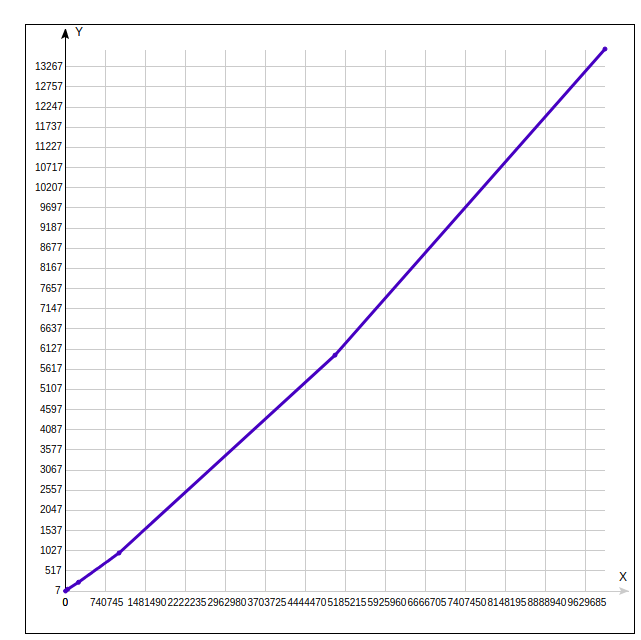
\includegraphics[scale=0.7]{graph.png}
\end{center}

По оси X отмечено количество данных, по оси Y -- время в миллисекундах. Как можно видеть, график почти линейный.

\subsection*{Недочёты}

Существуют более совершенные методы решения данной задачи, а так же более совершенные структуры данных, для ее решения, которые я, к сожалению, не смог реализовать.

\subsection*{Выводы}

Данный алгоритм, естественно, при должной реализации, имеет множество применений в практическом программировании. В силу своей скорости выполнения, вполне может применяться в областях программирования, работающах с большимим объемами данных. 

Например, сущетвует государственная база данных, сохраняющая списки автомобилистов. Здесь в качестве ключа может выступать, например, дата последнего участия в ДТП. И, таким образом, страховая компания может понять для себя риски в страховании того или иного человека.

Данный алгоритм в своем простейшем виде довольно прост для реализации, однако существуют, более сложные для написания реализации, но работающие заметно лучше. Так же можно найти незначительные улучшения в частных случаях работы алгоритма (как раз на примере автомобильных номеров в качестве ключей), что, впрочем, мне не очень-то удалось.

В ходе работы над данной задачей, основные трудности возникли с реализацией более оптимальных структур данных, для промежуточного хранения, не сильно замедляющих алгоритм частыми системнымим вызовами для аллокации памяти на куче.

\end{document}
